% !TEX root = ../../presentation.tex
% Core

\begin{slide}{MemoryValue}
\scalebox{1.0}{
  \begin{tabular}{l}
    \texttt{std::bitset}\\\\
    \texttt{boost::dynamic\_bitset}\\\\
    \texttt{std::vector\textless char\textgreater}\\\\
    \texttt{std::vector}\textless bool\textgreater\\\\
  \end{tabular}
  }
\end{slide}

\begin{slide}{MemoryValue}
\scalebox{1.0}{
  \begin{tabular}{l|c}
    & read and write single bits\\
    \texttt{std::bitset} & $\checkmark$ \\
    \texttt{boost::dynamic\_bitset} & $\checkmark$ \\
    \texttt{std::vector\textless char\textgreater} & $\times$ \\
    \texttt{std::vector}\textless bool\textgreater & $\checkmark$ \\
  \end{tabular}
  }
\end{slide}

\begin{slide}{MemoryValue}
\scalebox{1.0}{
  \begin{tabular}{l|c}
    & read and write single bytes\\
    \texttt{std::bitset} & $\times$ \\
    \texttt{boost::dynamic\_bitset} & $\times$ \\
    \texttt{std::vector\textless char\textgreater} & $\checkmark$ \\
    \texttt{std::vector}\textless bool\textgreater & $\times$ \\
  \end{tabular}
  }
\end{slide}

\begin{slide}{MemoryValue}
\scalebox{1.0}{
  \begin{tabular}{l|c}
    & read and write subStrings\\
    \texttt{std::bitset} & $\times$ \\
    \texttt{boost::dynamic\_bitset} & $\times$ \\
    \texttt{std::vector\textless char\textgreater} & $\checkmark$ \\
    \texttt{std::vector}\textless bool\textgreater & $\checkmark$ \\
  \end{tabular}
  }
\end{slide}

\begin{slide}{MemoryValue}
\scalebox{1.0}{
  \begin{tabular}{l|c}
    & determine size at construction time\\
    \texttt{std::bitset} & $\times$ \\
    \texttt{boost::dynamic\_bitset} & $\checkmark$ \\
    \texttt{std::vector\textless char\textgreater} & $\checkmark$ \\
    \texttt{std::vector}\textless bool\textgreater & $\checkmark$ \\
  \end{tabular}
  }
\end{slide}

\begin{slide}{MemoryValue}
\scalebox{0.65}{
  \begin{tabular}{l|cccc}
    & rw-single-bit & rw-single-byte & rw-subString & constructionTime-size \\\\
    \texttt{std::bitset} & $\checkmark$ & $\times$ & $\times$ & $\times$ \\\\
    \texttt{boost::dynamic\_bitset} & $\checkmark$ & $\times$ & $\times$ & $\checkmark$ \\\\
    \texttt{std::vector\textless char\textgreater} & $\times$ & $\checkmark$ & $\checkmark$ & $\checkmark$ \\\\
    \texttt{std::vector}\textless bool\textgreater & $\checkmark$ & $\times$ & $\checkmark$ & $\checkmark$ \\\\
    \texttt{MemoryValue} & $\checkmark$ & $\checkmark$ & $\checkmark$ & $\checkmark$ \\\\
  \end{tabular}
  }
\end{slide}

\begin{slide}{conversions}
  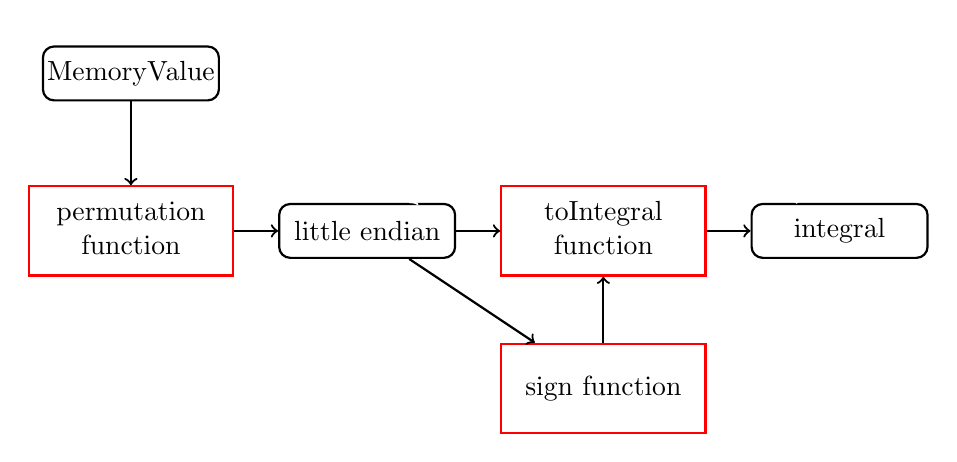
\begin{tikzpicture}[thick]

    \tikzset{block/.style={%
      draw,%
      rectangle,%
      rounded corners,%
      text width=2cm,%
      text height=0.45cm}%
    };
    \tikzset{reck/.style={%
      draw,%
      rectangle,%
      text width=2.36cm,%
      text height=0.9cm}%
    };

    \tikzset{smallblock/.style={block, text width=1.5cm, text height=0.3cm}};

    %%%%%%%%%%%%%%%
    % conversions %
    %%%%%%%%%%%%%%%
    \path (-9, 2) coordinate [block] (mvae) node {MemoryValue};

    \path[draw=red] (-9, 0) coordinate [reck] (perm) node {
      \begin{tabular}{c}
        permutation \\ function
      \end{tabular}
    };

    \path (-6, 0) coordinate [block] (mvle) node {little endian};

    \path[draw=red] (-3, -2) coordinate [reck] (sf) node {sign function};

    \path[draw=red] (-3, 0) coordinate [reck] (ti) node {
    \begin{tabular}{c}
      toIntegral \\ function
    \end{tabular}
    };

    \path[draw=white] (-3, 2) coordinate [reck] (tmv) node {};

    \path (0, 0) coordinate [block] (inte) node {integral};

    \draw [->] (mvae) -- (perm);
    \draw [->] (perm) -- (mvle);
    \draw [->] (mvle) -- (sf);
    \draw [->] (mvle) -- (ti);
    \draw [->] (sf) -- (ti);
    \draw [->] (ti) -- (inte);
    \draw[draw=white] [->] (inte) -- (tmv);
    \draw[draw=white] [->] (tmv) -- (mvle);

  \end{tikzpicture}
\end{slide}

\begin{slide}{conversions}
  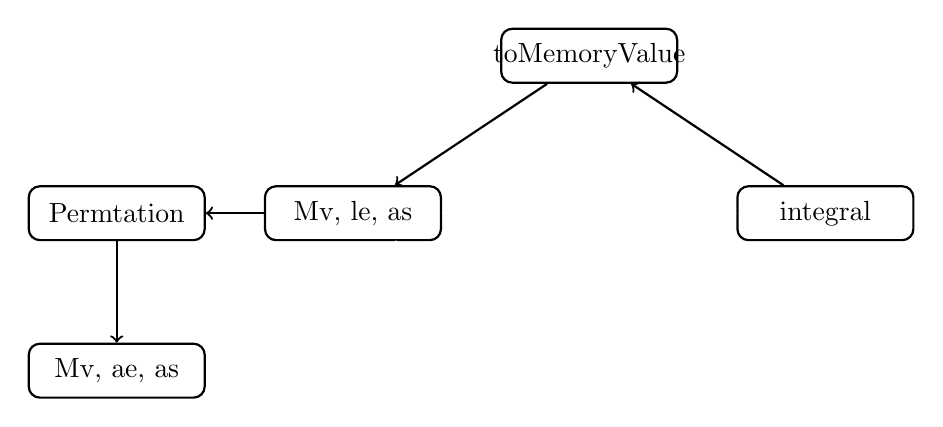
\begin{tikzpicture}[thick]

    \tikzset{block/.style={%
      draw,%
      rectangle,%
      rounded corners,%
      text width=2cm,%
      text height=0.45cm}%
    };

    \tikzset{smallblock/.style={block, text width=1.5cm, text height=0.3cm}};

    %%%%%%%%%%%%%%%
    % conversions %
    %%%%%%%%%%%%%%%
    \path (-9, -1.8) coordinate [block] (mvae) node {Mv, ae, as};

    \path (-9, 0.2) coordinate [block] (perm) node {Permtation};

    \path (-6, 0.2) coordinate [block] (mvle) node {Mv, le, as};

    \path[draw=white] (-3, -1.8) coordinate [block] (sf) node {};

    \path[draw=white] (-3, 0.2) coordinate [block] (ti) node {};

    \path (-3, 2.2) coordinate [block] (tmv) node {toMemoryValue};

    \path (0, 0.2) coordinate [block] (inte) node {integral};

    \draw [<-] (mvae) -- (perm);
    \draw [<-] (perm) -- (mvle);
    \draw[draw=white] [->] (mvle) -- (sf);
    \draw[draw=white] [->] (mvle) -- (ti);
    \draw[draw=white] [->] (sf) -- (ti);
    \draw[draw=white] [->] (ti) -- (inte);
    \draw [->] (inte) -- (tmv);
    \draw [->] (tmv) -- (mvle);

  \end{tikzpicture}
\end{slide}

\begin{slide}{register}
  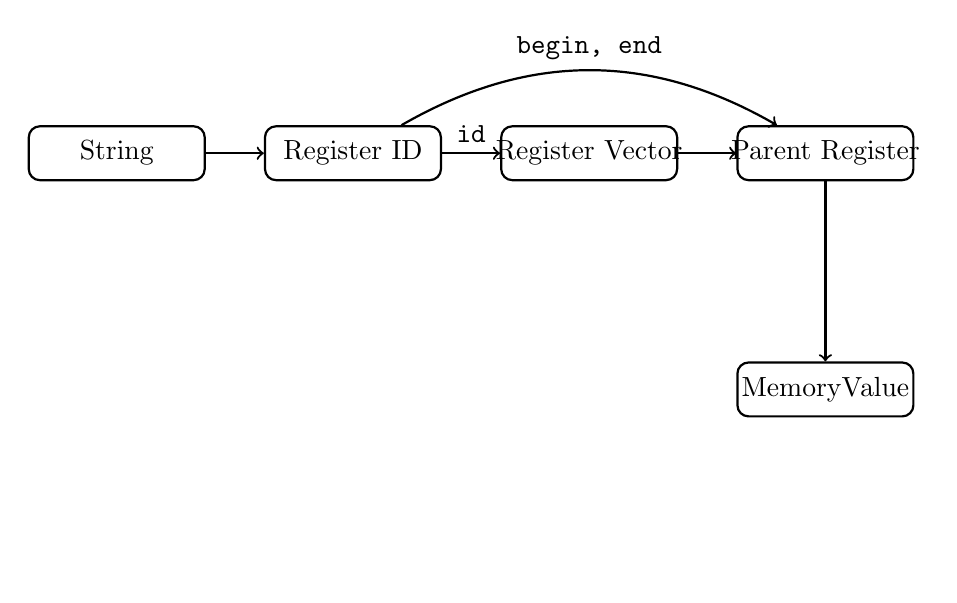
\begin{tikzpicture}[thick]

    \tikzset{block/.style={%
      draw,%
      rectangle,%
      rounded corners,%
      text width=2cm,%
      text height=0.45cm}%
    };

    \tikzset{smallblock/.style={block, text width=1.5cm, text height=0.3cm}};

    %%%%%%%%%%%%%%%
    %  register   %
    %%%%%%%%%%%%%%%
    \path (-4.5, 0) coordinate [block] (str) node {String};
    \path (-1.5, 0) coordinate [block] (rid) node {Register ID};
    \path (1.5, 0) coordinate [block] (rvc) node {Register Vector};
    \path (4.5, 0) coordinate [block] (pre) node {Parent Register};
    \path (4.5, -3) coordinate [block] (mvl) node {MemoryValue};
    \path[draw=white] (-4.5, -3) coordinate [block] (white) node {};
    \path[draw=white] (4.5, -5) coordinate [block] (white) node {};

    \draw [->] (str) -- (rid);
    \draw [->] (rid) -- (rvc) node [midway, above] {\texttt{id}};
    \draw [->] (rvc) -- (pre);
    \draw [->] (rid) to [out=30,in=150] node [midway, above] {\texttt{begin, end}} (pre);
    \draw [->] (pre) -- (mvl);

  \end{tikzpicture}
\end{slide}

\begin{slide}{register}
  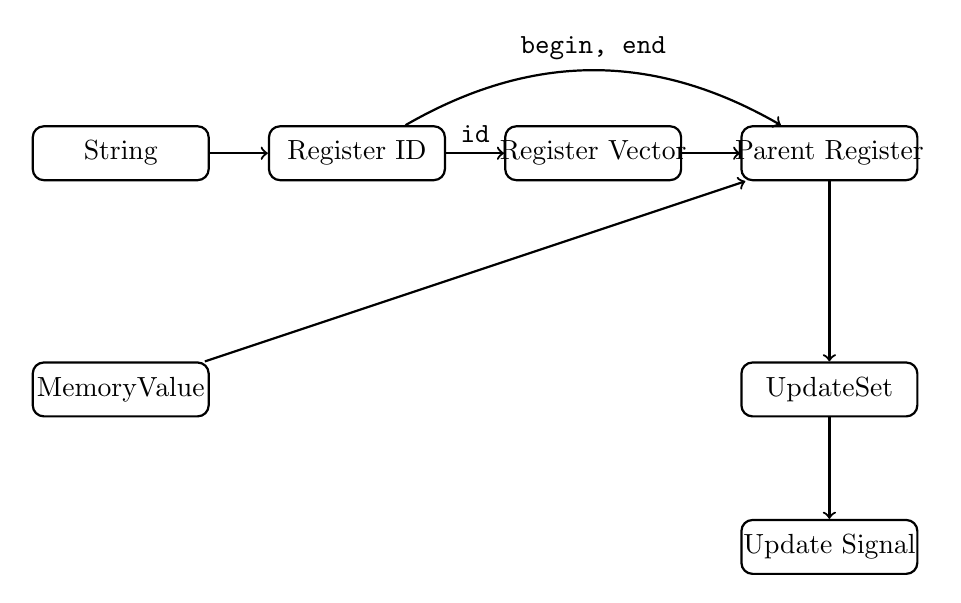
\begin{tikzpicture}[thick]

    \tikzset{block/.style={%
      draw,%
      rectangle,%
      rounded corners,%
      text width=2cm,%
      text height=0.45cm}%
    };

    \tikzset{smallblock/.style={block, text width=1.5cm, text height=0.3cm}};

    %%%%%%%%%%%%%%%
    %  register   %
    %%%%%%%%%%%%%%%
    \path (-4.5, 0) coordinate [block] (str) node {String};
    \path (-1.5, 0) coordinate [block] (rid) node {Register ID};
    \path (1.5, 0) coordinate [block] (rvc) node {Register Vector};
    \path (4.5, 0) coordinate [block] (pre) node {Parent Register};
    \path (-4.5, -3) coordinate [block] (mvl) node {MemoryValue};
    \path (4.5, -3) coordinate [block] (ups) node {UpdateSet};
    \path (4.5, -5) coordinate [block] (sig) node {Update Signal};

    \draw [->] (str) -- (rid);
    \draw [->] (rid) -- (rvc) node [midway, above] {\texttt{id}};
    \draw [->] (rvc) -- (pre);
    \draw [->] (rid) to [out=30,in=150] node [midway, above] {\texttt{begin, end}} (pre);
    \draw [->] (mvl) -- (pre);
    \draw [->] (pre) -- (ups);
    \draw [->] (ups) -- (sig);

  \end{tikzpicture}
\end{slide}

\begin{slide}{MemoryValue}
\scalebox{0.65}{
  \begin{tabular}{l|cccc}
    $\times$ & rw-single-bit & rw-single-byte & rw-subString & constructionTime-size \\
    \texttt{std::vector}\textless bool\textgreater & $\checkmark$ & $\times$ & $\checkmark$ & $\checkmark$ \\
    \texttt{boost::dynamic\_bitset} & $\checkmark$ & $\times$ & $\times$ & $\checkmark$ \\
    \texttt{std::bitset} & $\checkmark$ & $\times$ & $\times$ & $\times$ \\
    \texttt{std::vector\textless std::uint8\_t\textgreater} & $\times$ & $\checkmark$ & $\checkmark$ & $\checkmark$ \\
    \texttt{magic} & $\checkmark$ & $\checkmark$ & $\checkmark$ & $\checkmark$ \\
  \end{tabular}
  }
\end{slide}
